\documentclass[a4paper,14pt]{article}

\usepackage{comment} % Para comentar várias linhas ao mesmo tempo

%matemática
\usepackage{amsmath}
\usepackage{amssymb}

%diagramação
\usepackage{extsizes}
\everymath{\displaystyle}
\usepackage{geometry}
\usepackage{fancyhdr}
\usepackage{multicol}
\usepackage{graphicx}
\usepackage[brazil]{babel}
\usepackage[shortlabels]{enumitem}
\usepackage{cancel}
\usepackage{textcomp}
\usepackage{tcolorbox}

%tabelas
\usepackage{array} % Para melhor formatação de tabelas
\usepackage{longtable}
\usepackage{booktabs}  % Para linhas horizontais mais bonitas
\usepackage{float}   % Para usar o modificador [H]
\usepackage{caption} % Para usar legendas em tabelas
\usepackage{wrapfig} % Para usar tabelas e figuras flutuantes
\usepackage{xcolor} % Para cores do fundo de tabelas
\usepackage{colortbl} % Para cores do fundo de tabelas

%tikzpicture
\begin{comment}
	\usepackage{tikz}
	\usepackage{scalerel}
	\usepackage{pict2e}
	\usepackage{tkz-euclide}
	\usetikzlibrary{calc}
	\usetikzlibrary{patterns,arrows.meta}
	\usetikzlibrary{shadows}
	\usetikzlibrary{external}
\end{comment}


%pgfplots
\usepackage{pgfplots}
\pgfplotsset{compat=newest}
\usepgfplotslibrary{statistics}
\usepgfplotslibrary{fillbetween}

%colours
\usepackage{xcolor}



\columnsep=2cm
\hoffset=0cm
\textwidth=8cm
\setlength{\columnseprule}{.1pt}
\setlength{\columnsep}{2cm}
\renewcommand{\headrulewidth}{0pt}
\geometry{top=1in, bottom=1in, left=0.7in, right=0.5in}

\pagestyle{fancy}
\fancyhf{}
\fancyfoot[C]{\thepage}

\begin{document}
	
	\noindent\textbf{6FMA142 - Matemática} 
	
	\begin{center}Figuras semelhantes (Versão estudante)
	\end{center}
	
	\noindent\textbf{Nome:} \underline{\hspace{10cm}}
	\noindent\textbf{Data:} \underline{\hspace{4cm}}
	
	%\section*{Questões de Matemática}
	
	\begin{multicols}{2}
	    \noindent Figuras semelhantes são aquelas cujos tamanhos podem ter sido modificados, mas os ângulos continuam congruentes e as medidas ficam proporcionais.
		\noindent\textsubscript{--------------------------------------------------------------------------}
		\begin{enumerate} 
			\item No quadro a seguir, temos alguns desenhos que representam objetos reais ou figuras geométricas. Para cada um deles, diga se a figura possui alguma outra representação congruente ou semelhante (ou ambas). Nos casos em que você acha que isso não pode acontecer, tente explicar por quê. \\
			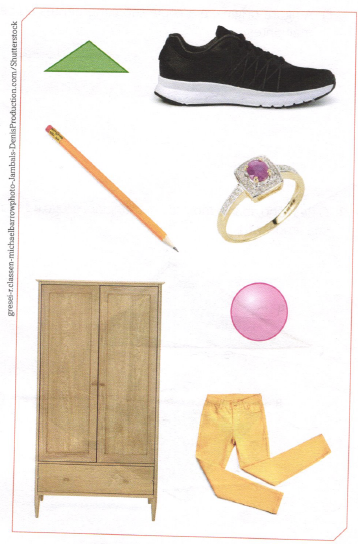
\includegraphics[width=1\linewidth]{6FMA142_imagens/imagem1}
			 \\
			\item Desenhe, numa folha à parte, usando régua e transferidor, um triângulo cujos ângulos internos medem 55°, 60° e 65°. Recorte esse triângulo e compare-o com os de seus colegas. Que conclusão podemos tirar dessa comparação? Justifique. \\\\\\\\\\\\\\\\\\\\
			\item Pense em 2 dados de um jogo de tabuleiro. Eles podem ser congruentes, semelhantes ou totalmente diferentes. Por quê? Faça a mesma análise com uma bola. \\\\\\\\\\\\\\\\\\\\\\
			%74 a 78
			\item No desenho a seguir temos vários retângulos. Como você já sabe, todos os ângulos dos retângulos são congruentes, pois todos são retos (90°). Entretanto, apenas dois deles são semelhantes. Assinale-os. \\\\\\\\\\\\\\\\\\\\
			\item O triângulo de vértices $A, B e C$ é semelhante ao triângulo de vértices $A', B'$ e $C'$, nessa ordem. O que você pode dizer sobre: 
			\begin{enumerate}[a)]
				\item $AB, AC, BC, A'B', A'C'$ e $B'C'$? \\\\\\\\\\\\\\\\
				\item $\hat{A}, \hat{B}, \hat{C}, \hat{A}', \hat{B}'$ e $\hat{C}'$ \\\\\\\\\\\\\\\\
			\end{enumerate}
			\item Por que todos os triângulos equiláteros são semelhantes? \\\\\\\\\\\\\\\\
			\item Por que todos os triângulos isósceles são semelhantes? \\\\\\\\\\\\\\\\
			\item Por que todos os cubos são semelhantes? \\\\\\\\\\\\\\\\
		\end{enumerate}
		$~$ \\ $~$ \\ $~$ \\ $~$ \\ $~$ \\ $~$ \\ $~$ \\ $~$ \\ $~$ \\ $~$
	\end{multicols}
\end{document}